\documentclass[../physical_computing.tex]{subfiles}

\begin{document}

\chapter{Lab Exercise 8 - Asynchronous Shared Memory}
\label{sec:appendix_8}

The lab exercise in Appendix \ref{sec:appendix_7} was a simple ``Hello, world!'' program. Whilst this made successful use of the soft Microblaze core on the FPGA, it is pretty clear that this kind of computer is in all ways inferior to the laptops I lent you at the beginning of the course! To make successful use of soft cores, they must be able to interact with devices that we build in programmable logic on the FPGA chip. As alluded to in the seminars, there are two main categories of interaction. These are the exchange of data, which can be achieved using shared memory, and the sending of signals, which can be achieved using interrupts. In this exercise, we will use shared memory. 

Shared memory is exactly what it says on the tin. Computers operate through the storage of programs and data in memory. This memory is accessed using a memory map. Each memory element has an address, and the addresses are usually expressed as numbers written, at the time of writing, as 32 bit binary numbers. Rather than writing out 32 1's and 0's, which would be arduous and error-prone, we adopt the only-slightly-better convention of representing these 32 bit numbers 8, 4-bit 'words', where a 4 bit word is represented as a single digit in hexadecimal, for example \texttt{0xC0000000}. In binary, this particular address is \texttt{b11000000000000000000000000000000}; you can see why binary representation is inconvenient. At least some of the memory addresses available to the processor can be used for the storage of data; you can write data to those addresses using a mechanism called pointers, which I will explain in a subsequent section, and read the data back from that same address into your program.

Shared memory provides a set of memory addresses to be written to, and read by, both the processor core and the programmable logic. The word asynchronous means that the shared memory is protected from a potential problem called a race condition. A race condition arises if both the processor and the programmable logic try to write to the shared memory at the same time, or if one tries to write whilst the other one simultaneously tries to read. If this happens, one of the two accessors is allowed to go first, and the other waits until it has finished. This queuing is handled by the shared memory hardware, and it is not possible to predict which of the processor the shared memory will perform its operation first. If it matters, then you must exercise tighter control of writing and reading to shared memory. This can be accomplished, for example, by the use of interrupts.

\section{New `IP' Devices}
\label{sec:appendix_8_devices}

The hardware I would like you to build today starts with the same layout that we used in the previous lab. You have a microblaze core connected to memory and a UART interface connected to a terminal. But, this time, we add some additional elements that are used to configure some shared memory. These make use of several new parts from the Xilinx IP catalogue, described below.

\subsection{Constant}
\label{sec:appendix_8_constant}

This element simply outputs a constant value. You can find it by using the "+" button in the diagram and searching for `Constant'. If you right-click on the block and select `Customize block', there are two parameters you can set, the width of the constant in bits, and the value of the constant. The value of the constant can be written in decimal, or in binary using \texttt{0b1111} for 15, for example, or in hexadecimal using \texttt{0xf} for the same number in hexadecimal.

\subsection{Concat}
\label{sec:appendix_8_concat}

This element allows you to join together two or more buses to make one big one that has width equal to the sum of the widths of the input buses. You can customise the block to set the number of buses you wish to concatenate and the width of each of the buses.

\subsection{Slice}
\label{sec:appendix_8_slice}

This element allows you to extract a sub-range of the bits from a bus. For example, if you have a 32 bit bus coming in, you might want an output bus that is bits 0 to 15 inclusive of the input bus. Customising slice allows you to specify the width of the input bus, and the subset of the bits from the input bus you wish to write to the output bus. The width of the output bus is automatically the number of bits in the range you specify, which is inclusive of the elements specified at both ends.

\subsection{Block Memory Generator}
\label{sec:appendix_8_block_memory}

This element generates the shared memory. It arrives by default with one input port. There are many configuration paramters on customisation. The most important one is in the `Basic' tab and it is `Memory Type'. We will always set this to `True Dual Port RAM'. This is the only element that you will need to specify. When the customised block appears in your diagram, you can click on the '+' icon next to either of the `BRAM\_PORT' inputs to see what is included in these buses. Each one has various inputs and outputs. We will typically operate the BRAM with port A connected to the processor system by way of a BRAM controller (to be described next), so that we won't need to break out the sub-components of this port, and port B connected to the programmable logic, so we will need to define the inputs and outputs to the sub-elements of that port.

\subsection{AXI BRAM Controller}
\label{sec:appendix_8_bram_controller}

Shared memory is connected to the processor system using a general purpose, and quite sophisticated, bus called AXI4. Both the shared memory and the controller for the UART port that connects to your terminal are on this same bus, and once you have more than one device connected to the AXI port, this in turn leads to a requirement for yet another piece of IP called AXI SmartConnect. Fortunately, if you put both the UARTlite and the AXI BRAM Controller IP on the same diagram, 'Run Connection Automation' will automatically connect everything up using AXI SmartConnect and it should all work. 

Using these new pieces of IP, and the Microblaze processor we used last time, we will build the hardware necessary for the project.

\section{Building the Hardware}
\label{sec:appendix_8_hardware}

The full hardware configuration we are going to build today is shown in Figure \ref{fig:appendix_8_hardware}. Build the diagram up using the instructions below. Some of the blocks that you will add will need to be customised. Customisation of the various blocks is described in Section \ref{sec:appendix_8_devices}.

\begin{enumerate}
    \item Open the hello world project from last time. The block diagram should look like that in Figure \ref{fig:appendix_8_prereq}. Exit Vitis.
    \item Check that it still works! Run the hello world program, open the terminal, and verify that you get the greeting. Note that the constraint file should have the clock and reset buttons uncommented, and that the names of those ports in the constraint file should match the names appearing in the diagram. 
    \item In vivado, from the File menu, select Project, then `Save As...'. Select a folder to put it in, and ensure that the option to create a new subfolder for the project is checked, then name your project, perhaps `sharedmemory'. This should automatically migrate you into the new `sharedmemory' project area, leaving the hello world project unchanged.
    \item Import the `Block Memory Generator', customising as described in Section \ref{sec:appendix_8_block_memory}. Break out port B using the `+' icon so you can see all the sub-ports of this bus.
    \item Import the 'AXI BRAM Controller'. Customise the AXI Bram controller to reduce the number of BRAM interfaces to from 2 to 1. This turned out to be critical to getting it to work, so be sure to do this.
    \item Move both the new IPs down to the lower part of the diagram, below the Microblaze processor. This will make it easier to wire in the constants later.
    \item Select `Run Connection Automation'. This will bring up a set of check-boxes for the buses you want to connect. Select all except \texttt{BRAM\_PORTB}. Now click on the button at the top of the diagram pane that looks like a step with a circular arrow inset. This should neaten up the diagram, and it should look like that shown in Figure \ref{fig:appendix_8_afterbram}. It does not matter if everything is not in exactly the same place, so long as the wires are connected to all the peripherals. 
    \item In the file menu, save the block design. You never know when things might crash.
    \item In the constraints file, un-comment the switches and LEDs and save the file. 
    \item Wire the \texttt{clkb} port on the block memory generator to any of the other wires connected to \texttt{clk} in the diagram. Get two Constants from the IP catalog, and set them to single bit binary 1 and binary 0, respectively. Wire the binary 1 to the \texttt{enb} (enable b) port, and the binary 0 to the \texttt{rstb} (reset) port.
    \item Save the block design again.
    \item Get a \texttt{Slice} IP. Customise it so that the highest 16 bits are extracted from a 32 bit buffer. Connect its input to \texttt{doutb} from the block memory. Right click on its output and select 'Make external'. Change the name of the external port to \texttt{led} to match the led outputs in the constraint file.
    \item Get a \texttt{Concat} IP. Customise so that it concatenates together two 16 bit buses into a 32 bit one. You will need to toggle the switches for the widths of the input ports from auto to manual and set them both to 16. There should now be two input ports to the Concat, called \texttt{In0} and \texttt{In1}. The \texttt{In0} port should be made external and renamed to \texttt{sw} to match the switches. The \texttt{In1} port should be connected to a sixteen bit wide constant whose value is zero. Connect the 32 bit wide output bus from the \texttt{Concat} IP to \texttt{dinb} on the Block Memory Generator.
    \item Save your diagram again.
    \item Import another constant. This should be set to 32 bits wide and a value of 0. Wire this constant to the \texttt{addrb} input to the block memory generator. This defines which memory address is being connected to, relative to the base address of the block memory. We are using the very first address, so the memory offset into the address space of the block memory is zero.
    \item The last port to wire on the block memory is the \texttt{web} port. This is short for write enable. It has 4 bits, each of which corresponds to one of the four bytes in the 32-bit-wide field of data to and from the device. We are here always writing the lowest 16 bits from the switches into the block memory, and writing the highest 16 bits from the block memory to the LEDs. So, we set these bits to \texttt{0b0011}, so that the lowest 16 bits are `write enabled'; we can write the memory corresponding to these bits into the shared memory device.
    \item Save your diagram, which should now have the same connections as shown in Figure \ref{fig:appendix_8_hardware}.
    \item Run synthesis, run implementation and build the bitstream file as usual. This takes a while because there are many IP cores in this project. Be patient. However, be warned that when I tried this Vivado quit half way through. This left a bunch of zombie processes running - if this happens to you, you can see the zombie processes in a shell window by invoking \texttt{ps -ef | grep Vivado}. In this position, having no idea whether these processes were actually doing anything useful, I decided to restart my laptop and re-open vivado. Vivado attempted to re-launch the build, but I decided to terminate this and re-start the synthesis process. This did finally build everything, but I'm telling you because it was a bit arduous and stressful, so you don't worry if the same thing happens to you.
    \item As for the hello world example, Use File, Export, Export hardware to export the hardware description file. To avoid confusing it with the other ones, rename the file shared\_memory, rather than design\_1\_wrapper.
    \item Connect the board to your laptop and power it on, ready to be programmed.
\end{enumerate}

\begin{figure}
    \centering
    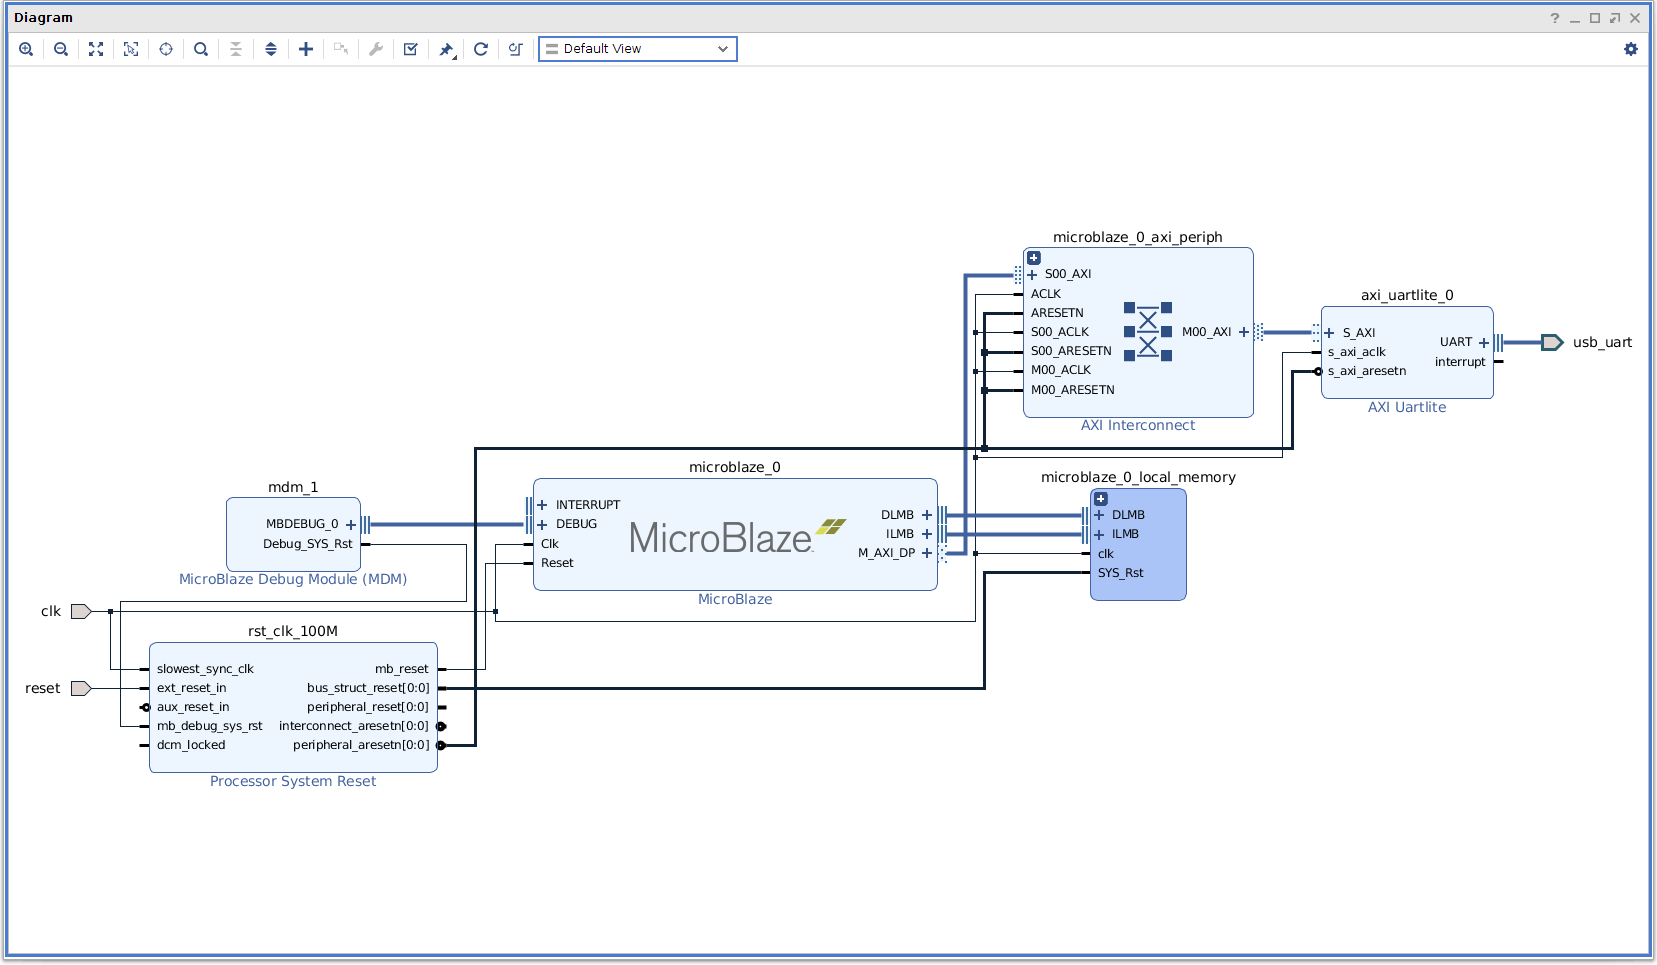
\includegraphics[width=\textwidth]{appendix_9/figures/prereq_diagram.png}
    \caption{The diagram for the `Hello World' project.}
    \label{fig:appendix_8_prereq}
\end{figure}

\begin{figure}
    \centering
    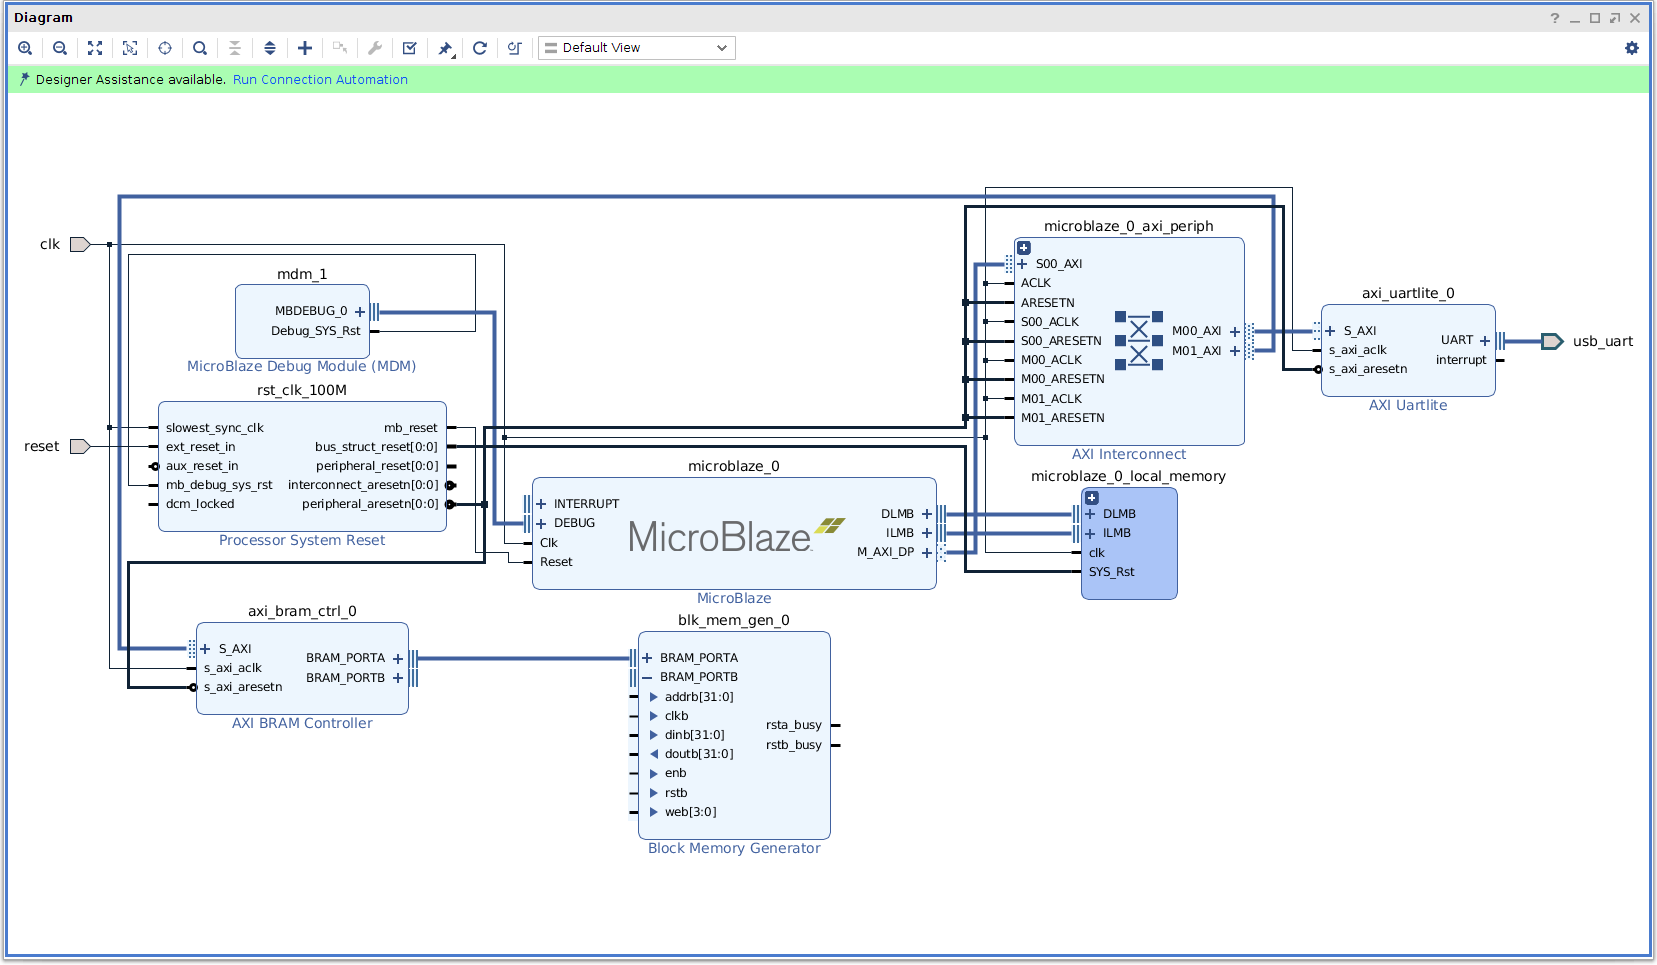
\includegraphics[width=\textwidth]{appendix_9/figures/after_bram.png}
    \caption{The shared memory hardware after the shared memory and controller are connected using block automation.}
    \label{fig:appendix_8_afterbram}
\end{figure}

\begin{figure}
    \centering
    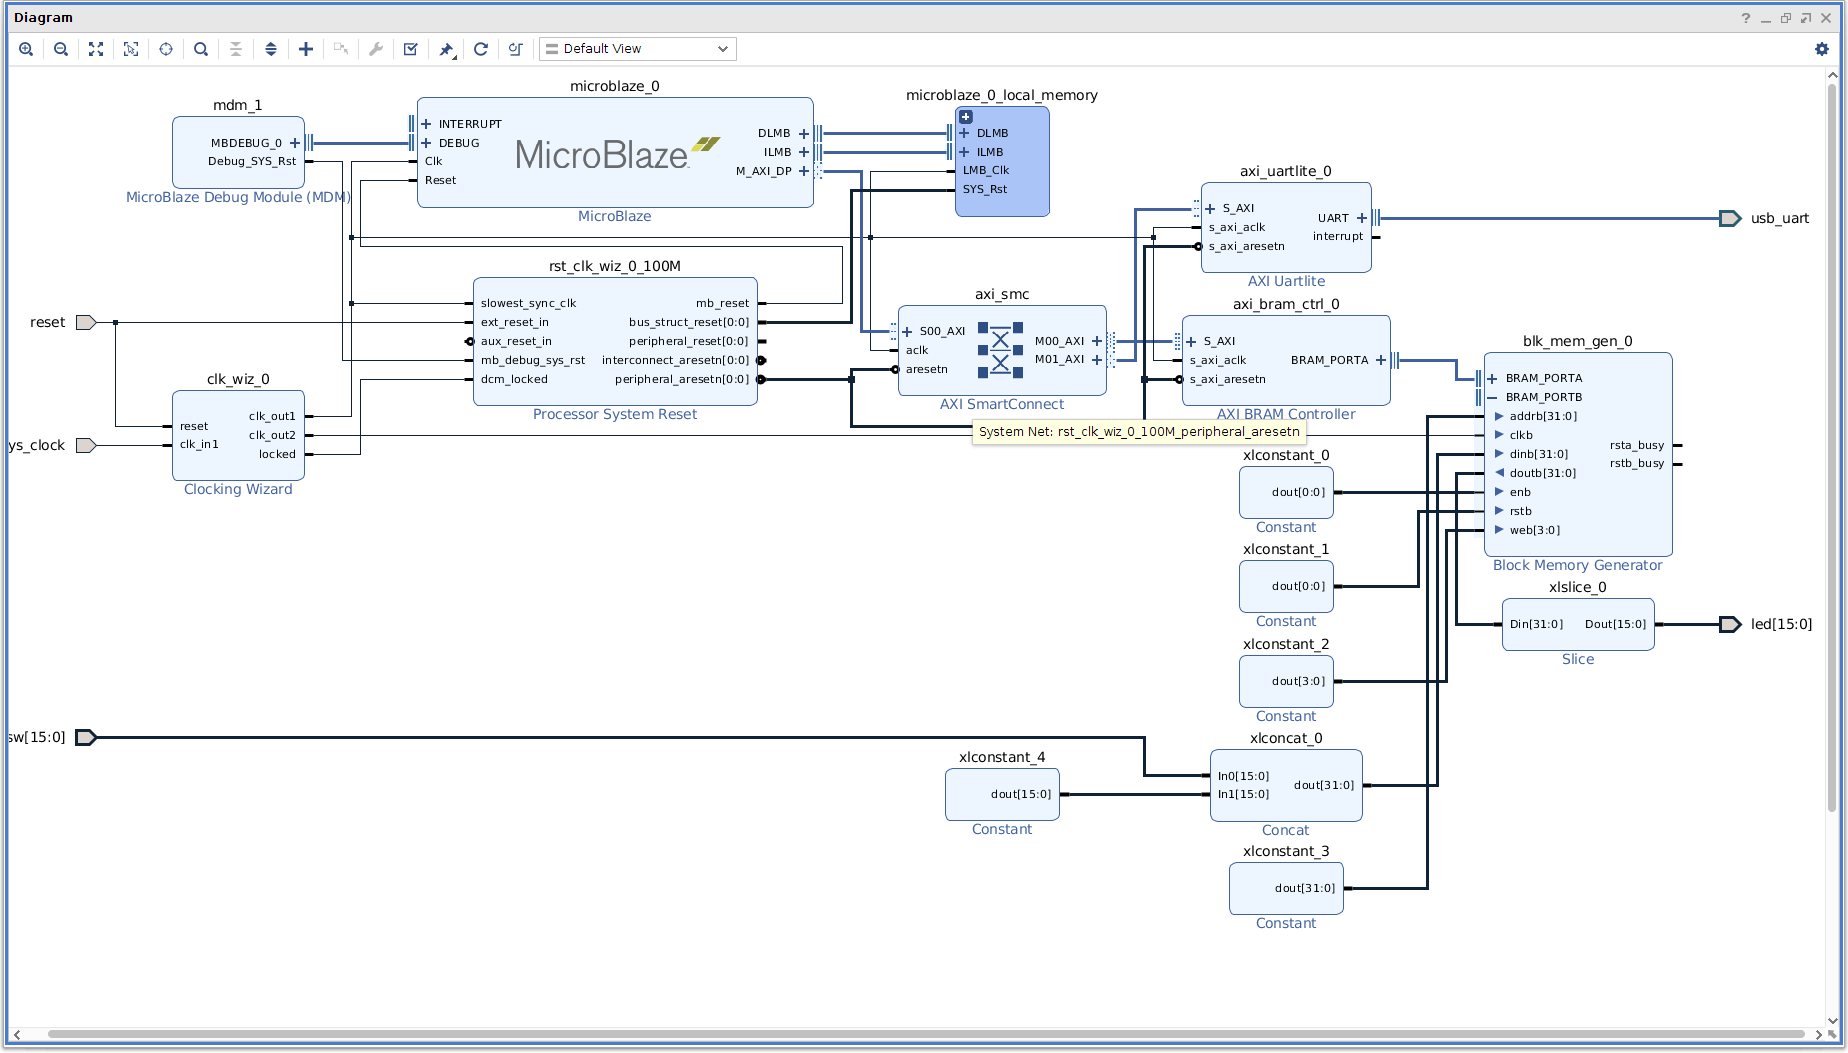
\includegraphics[width=\textwidth]{appendix_9/figures/full_diagram.png}
    \caption{The block diagram for the shared memory exercise.}
    \label{fig:appendix_8_hardware}
\end{figure}

\section{C code for the shared memory}

You should start a new Vitis project based on the hello world template just as you did last time. However, the hello world code should be replaced by a copy of the code segment below.

\newpage

\begin{minted}{c}
#include <stdio.h>
#include <unistd.h>
#include "platform.h"
#include "xil_printf.h"
#include <xparameters.h>

int main()
{
	u16* pdataval=(u16*)XPAR_BRAM_0_BASEADDR;
	u32 counter=0;
    init_platform();

    pdataval[1]=127+32768;
    while(1) {
    	xil_printf("count %u, value %u\r\n",counter++,pdataval[0]);
    	sleep(1);
    }

    cleanup_platform();
    return 0;
}
\end{minted}

This code contains several elements requiring explanation. First, the new include file \texttt{<xparameters.h>}. This file is produced by Vivado, and defines the memory
map of the hardware we just built. This memory map includes an address for the start of the shared memory block. This is needed here, because we are going to both read
from and write to the shared memory in this code. The address is defined as a preprocessor `constant', written \texttt{XPAR\_BRAM\_0\_BASEADDR}. It's actual value in 
the code is \texttt{0xC0000000}. 

In the \texttt{main} program, we first define a couple of constants, but we do it using a new and interesting syntax in the very first line,

\begin{minted}{c}
u16* pdataval=(u16*)XPAR_BRAM_0_BASEADDR;
\end{minted}

This means that pdataval is the {\it address of} a variable of type u16. This is the first example that you have met of the use of a pointer. A pointer in C is just an address in the memory of the computer. The value of this address is \texttt{0xC0000000}, and it corresponds to the address in memory where the shared memory starts. The other variable is just a counter used in the loop below.

The next interesting thing is this line:

\begin{minted}{c}
pdataval[1]=127+32768;
\end{minted}

pdataval is an address at the short integer, 16 bits in size. pdataval[0] is the {\it value at} this memory location. We just set this to 127+32768. The binary bit pattern of this is
\texttt{0b1000000001111111}. This is what your LED outputs should display. This is your first write from the processor system to the LED outputs. 

Next we enter an infinite loop, using the standard code for setting up infinite loops, 
\texttt{while(1)}. Everything inside the curly braces after this statement repeats until the board is switched off. This code prints the value of a counter, followed by the value at address (or pointer) pdataval. This value is set from the switches in the hardware. So, if you change the switches, you should see the value printed out change in your terminal when this code is running.

Here are the instructions for the rest of the project.

\begin{enumerate}
    \item Launch vitis. Either make the base directory the same as your vivado project directory containing your .xsa file, or choose a new empty directory.
    \item Make a new project using your .xsa file to specify the hardware.
    \item Make a hello world project.
    \item In vivado, use the hardware manager to program the board.
    \item Open the serial comms program, open a connection to port USB1 at 9600 baud as you did last week.
    \item Run the hello world program as you did last week, check that Hello World appears in the terminal.
    \item Now replace the C code in helloworld.c with the code we just described. 
    \item Highlight the system directory and rebuild with the hammer icon.
    \item Highlight the directory under system containing your software application.
    \item Launch on the system. The LEDs should after a short delay display the bit pattern \texttt{0b1000000001111111}. The terminal should update once a second, and display the bit pattern set on the switches.
\end{enumerate}


\end{document}